% Source of the figure zz-walk.pdf. (a) The ZZ instance of the graph G_b: the chain u < b < a < v with the edges of R
% and the walk u, a, b, v in red; the dashed line separates D = {u, b} from the rest. (b) A valid walk of length seven:
% lows in the band L_P, highs in the band U_P, and a down-set D between them. Larger elements are drawn higher.
% Compile with pdfLaTeX; the PDF is included in the manuscript at its natural size.
\documentclass[tikz,border=1pt]{standalone}
\usepackage[T1]{fontenc}
\pdfinfoomitdate=1 \pdftrailerid{} \pdfsuppressptexinfo=-1
\definecolor{pathred}{RGB}{200,40,40}
\tikzset{
  vertex/.style={circle, fill=black, inner sep=0pt, minimum size=2.2mm},
  terminal/.style={circle, fill=black, inner sep=0pt, minimum size=3mm},
  edge/.style={line width=0.7pt},
  pathedge/.style={line width=1.8pt, pathred, line cap=round},
  band/.style={rounded corners=5pt, fill=gray!14, draw=gray!75!black, line width=0.6pt},
  cutline/.style={line width=0.7pt, dash pattern=on 4pt off 3pt, draw=black!70}}
\begin{document}
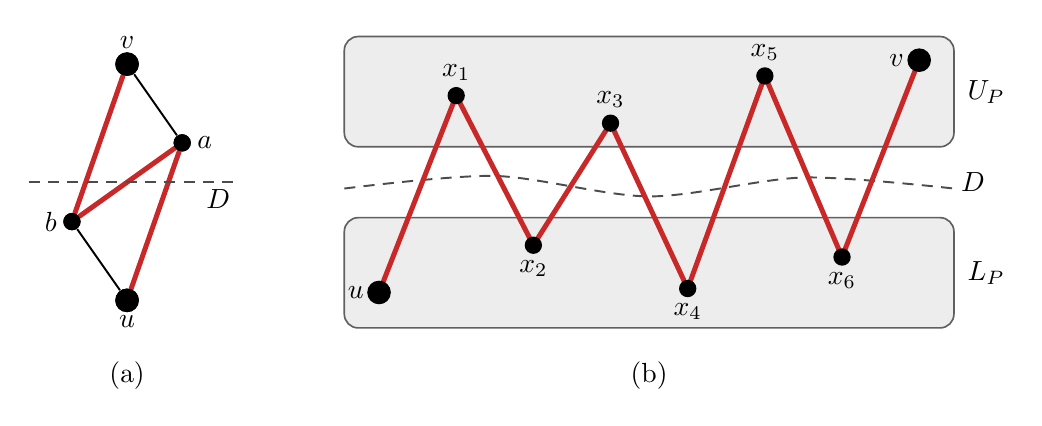
\begin{tikzpicture}[x=1cm, y=1cm]
  % panel (a)
  \begin{scope}
    \node[terminal] (u) at (0.7,0) {};
    \node[vertex]   (b) at (0,1.0) {};
    \node[vertex]   (a) at (1.4,2.0) {};
    \node[terminal] (v) at (0.7,3.0) {};
    \draw[edge] (u) -- (b) (a) -- (v);
    \draw[pathedge] (u) -- (a) -- (b) -- (v);
    \foreach \p/\s in {u/terminal, b/vertex, a/vertex, v/terminal} \node[\s] at (\p) {};
    \node[below=2pt] at (u) {$u$};
    \node[left=2pt]  at (b) {$b$};
    \node[right=2pt] at (a) {$a$};
    \node[above=2pt] at (v) {$v$};
    \draw[cutline] (-0.55,1.5) -- (2.05,1.5);
    \node[anchor=north east, inner sep=1pt] at (2.05,1.45) {$D$};
    \node at (0.7,-0.95) {(a)};
  \end{scope}
  % panel (b)
  \begin{scope}[xshift=3.9cm, x=0.98cm]
    \draw[band] (-0.45,-0.35) rectangle (7.45,1.05);
    \draw[band] (-0.45,1.95) rectangle (7.45,3.35);
    \node[anchor=west] at (7.5,0.35) {$L_P$};
    \node[anchor=west] at (7.5,2.65) {$U_P$};
    \draw[cutline] plot[smooth] coordinates {(-0.45,1.42) (1.5,1.58) (3.5,1.32) (5.5,1.56) (7.45,1.42)};
    \node[anchor=west, inner sep=1pt] at (7.5,1.5) {$D$};
    \coordinate (x0) at (0,0.1);
    \coordinate (x1) at (1,2.6);
    \coordinate (x2) at (2,0.7);
    \coordinate (x3) at (3,2.25);
    \coordinate (x4) at (4,0.15);
    \coordinate (x5) at (5,2.85);
    \coordinate (x6) at (6,0.55);
    \coordinate (x7) at (7,3.05);
    \draw[pathedge] (x0) -- (x1) -- (x2) -- (x3) -- (x4) -- (x5) -- (x6) -- (x7);
    \node[terminal] at (x0) {};
    \node[terminal] at (x7) {};
    \foreach \i in {1,...,6} \node[vertex] at (x\i) {};
    \node[left=2pt]  at (x0) {$u$};
    \node[left=2pt]  at (x7) {$v$};
    \node[above=2pt] at (x1) {$x_1$};
    \node[below=2pt] at (x2) {$x_2$};
    \node[above=2pt] at (x3) {$x_3$};
    \node[below=2pt] at (x4) {$x_4$};
    \node[above=2pt] at (x5) {$x_5$};
    \node[below=2pt] at (x6) {$x_6$};
    \node at (3.5,-0.95) {(b)};
  \end{scope}
\end{tikzpicture}
\end{document}
